% Chapter 3

\chapter{Data Generation and Analysis} % Main chapter title

\label{Data} % For referencing the chapter elsewhere, use \ref{Chapter1} 

%----------------------------------------------------------------------------------------
This chapter will address the methods and efforts to tackle the task of data generation as well as labeling the huge amount of data that was recorded.\\
It was the most time-consuming part of this work, since it involved a lot of postprocessing and data cleansing work that had been necessary due to the multi-modality of the recording devices and capturing data with different frequencies with various data formats which also were partly unsynchronized. Furthermore, methods that were used to label the generated data mostly automatically, based on position data of the hand and the MHSB, as well as a representation of the distribution of the stimuli objects on the frames, will be explained.

%----------------------------------------------------------------------------------------
\section{Data Structure and Requirements}
The data in this experiment was recorded with multiple devices, including the Vicon system, the 2 parts of the glove as well as 3 cameras, generating side- and top-views. In order to train a classifier with supervised learning, following requirements were made for the data:
%To be able to train a classifier with supervised learning, there were a number of requirements to the data:
\begin{enumerate}
\item Simultaneous data acquisition
\begin{itemize}
\item Capturing all devices at the same time will facilitate upcoming processing steps.
\end{itemize}
\item Postprocessing raw data
\begin{itemize}
\item To be able to work with the data, raw data needs to be processed and all files need to be in the same format.
\end{itemize}
\item Synchronizing the time-series
\begin{itemize}
\item Delays in the data acquisition and different device frequencies make this step necessary.
\end{itemize}
\item Generating the labels
\begin{itemize}
\item For supervised learning, the whole dataset needs to be labeled.
\end{itemize}
\end{enumerate}
%----------------------------------------------------------------------------------------
\section{Recording} \label{recording}
To aid recording the data of all devices at the same time and with only one start signal, a tool called Multiple Start Synchronizer (MSS) was used. MSS sends a trigger signal to all registered devices which makes them start and stop capturing data.\\
The Vicon and Basler camera data were captured directly within the Vicon Nexus program. For the glove, data was recorded as rosbag consisting of two topics for each part of the glove. Side-view camera images were captured directly as image files.\\
\\
Despite using MSS, there were still delays among the different devices that had to be synchronized separately. 
%----------------------------------------------------------------------------------------
\section{Postprocessing Vicon Data}
The first step in the pipeline was to postprocess the Vicon data. In this procedure, a three-dimensional hand model with marker positions was fitted to an image of the subjects hand (See Figure \ref{autotracker}, left). This model was then used to reconstruct the hand movement during the experiment with an autotracker tool \cite{autotracker} to approximate marker positions that occurred during gaps in the recording when no camera captured a marker  (See Figure \ref{autotracker}, right).\\
\\
The resulting file contains a time-series of the x-,y- and z-position of each marker. Furthermore a file with the joint-angles was generated.

\begin{figure}[h]
	%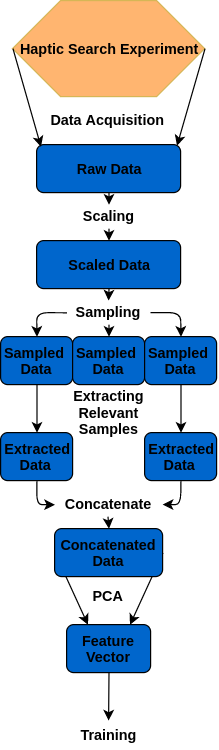
\includegraphics[scale]{Pipeline2}
	\makebox[\textwidth][c]{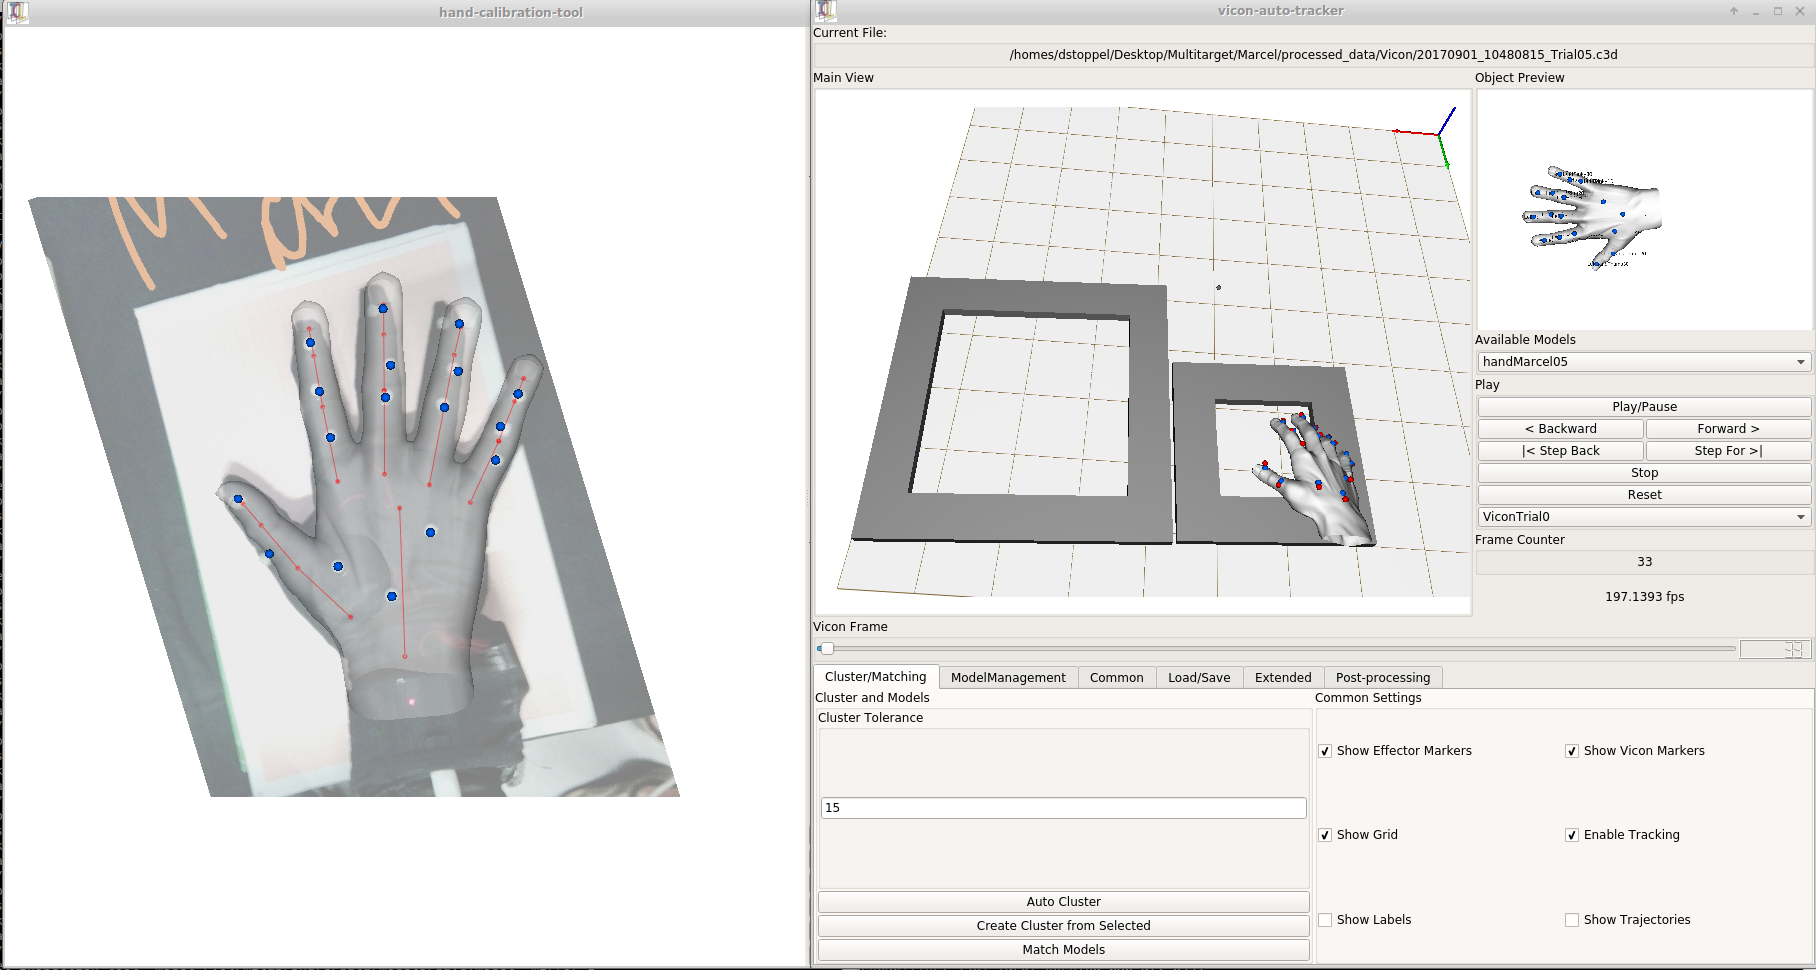
\includegraphics[scale=0.22]{reconstruction}}
	\caption{Fitting a hand model (left) and using it in the autotracker to fill gaps (right).}
	\label{autotracker}
\end{figure}
%----------------------------------------------------------------------------------------
\section{Generating Labels}
This section will describe the methodology that was used to generate labels for the recorded data. The challenge was to write a program, that will do most of the work automatically and handle the huge amount of data generated by this experiment.\\
With 7 subjects participating in up to 5 trials each, and time series containing between 5000 and 7000 data points for each trial, a manual labeling of the data would be too time-consuming. Also having to cope with unsynchronized data due to delays between the modalities would make this task hard to tackle without proper preprocessing. The solution was a program that used the trajectories of the Vicon data to extract objects that were explored during the search experiment and to label them appropriately. The exact procedure is described in the subsections below. It can be summarized to three mandatory steps:
\begin{enumerate}
	\item Synchronizing data from Vicon and glove to allocate positions to tactile data.
	\item Building a representation of the experimental setting to recreate it in sense of the hand trajectories and object distribution.
	\item Generating labels by replaying these trajectories and constructing a vector containing the explored objects at each timestep.
\end{enumerate}

\subsection{Synchronizing Glove and Vicon Data}
A problem that occurred during the acquisition was the delay between starting the Vicon system and the glove recording. Although it was sending a trigger signal to both systems at the same time, the glove started capturing data approximately 3 to 5 seconds later. Additionally the beginning of the Vicon data had to be cut by 100 to 1000 frames for postprocessing reasons. Fitting the three-dimensional model was only successful if the markers of the first frames had been in a nearly perfect plane position. Consequently, an offset had to be defined pointing to the beginning of the Vicon time series because the data only contains a timestamp describing the beginning of the recording. On the other hand, the recorded rosbags from the glove had a timestamp for each sample.\\
Since the frequency of the tactile glove with 150 Hz was lower than the frequency of Vicon with 200 Hz, the trajectory data had been reduced to the length of the tactile glove.\\
\\
Considering the two time series $V = \{v_{t} \mid t\in T_{V}\}$ and $G = \{g_{t} \mid t\in T_{G}\}$ that would describe the set for the Vicon data and glove data. The set of timestamps $T_{G}$ was given for the tactile data and consisted of unix time values. For $T_{V}$ the timestamps had to be calculated for each sample from the initial timestamp, the offset and the frequency. \\
To synchronize, a new time series $V' \subset V$ was defined with \begin{center}
$V' = \{v_{t} \mid \forall g_{t_{g}} \in G \exists v_{t_{v}} \in V : (t_{v} \geq t_{g}) \wedge (t_{v} < t_{g+1}), t_{v} \in T_{V}, t_{g} \in T_{G} \}$
\end{center}
This new time series has now equal length to $G$. Each time value from $V'$ matched exactly one time value from the time series $G$.
\subsection{Representing Glove and Objects}
The core idea behind this program was to use the trajectories of the hand and approximated object positions in order to detect which object was covered by the hand during which time. By having trajectory data acquired, the only thing that had to be done manually was the object distribution. For this, a representation of the board was generated in form of a matrix $B \in \mathbb{R}^{10 \times 10}$ for each trial. In this representation, $b_{11} \in \Omega=\{0,..,5\}$ would be the top left object and from there rows and columns were generated accordingly where $\Omega$ is the set of labels. To decrease the number of false-positives, only explored objects were considered in this representation.\\
The next level was to represent this information in a coordinate system by generating polygons for each object in $ B $ to embody the MHSB. Since only the top corners of the boards were assembled with markers, the positions for respective corners of the polygons had to be calculated based on this. First for each object $ b_{ij} \in B $ a polygon $ P_{ij} = \begin{pmatrix}a & b \\ c & d\end{pmatrix} $ was created where each element describes the x- and y-position of a corner. In the second step, this polygon was represented as its center position $ z = \begin{pmatrix}
z_{x} \\ z_{y}
\end{pmatrix}$. The result is a matrix $B' = \begin{pmatrix}
z_{11} & \hdots & z_{1n} \\
\vdots & \ddots & \vdots \\
z_{n1} & \hdots & z_{nn}
\end{pmatrix}$
that represents every object in $ B $ through a position.\\
\\
The remaining problem was that the top left position of the bigger frame was used as a base to build our polygons using a step size corresponding to the edge length of the stimuli. As a result, the represented board was placed parallel to the x- and y-axis into the coordinate system. Because this did not match the real setting, the matrix $ B' $ had to be rotated. For this the actual angle $ \alpha $ between the vector $\vec{t} = \mu_{tr} - \mu_{tl}$, where $\mu_{tl}$ is the mean position of the top left corner and $\mu_{tr}$ the mean position of the top right corner,  and the x-axis had to be calculated to build a rotation matrix $ R_{\alpha} $. The angle $\alpha$ describes the angle that was needed to rotate the representation so that the orientation of $ B' $ matches the one in the real setting. The final matrix for the stimuli representation is $ B''  = \begin{pmatrix}
 R_{\alpha}z_{11} & \hdots &  R_{\alpha}z_{1n} \\
\vdots & \ddots & \vdots \\
 R_{\alpha}z_{n1} & \hdots &  R_{\alpha}z_{nn}
\end{pmatrix}$.\\
\\
\\
With $ B'' $ a matrix was now given that could be used for assigning objects, or in this case their labels, to hand positions. But in order to do this, a representation for the hand had to be thought of. For now, the hand consisted of 17 trajectories $ t_{i} $, one for each marker $ i $. \\
A first approach was to use a convex hull $ H_{c} $ of the hand and check for each time step in $ V' $ if $ H_{c} $ contained points $ p \in B'' $. This idea was discarded quickly because the seize of the convex hull was to large, resulting in multiple possible objects $ p $ for each time step. Furthermore it was computationally costly since for every step the whole matrix $ B'' $ had to be checked for contained points. This led to an extension of $ B'' $ where a k-d-tree was build containing positions of all $p$ such that it could be efficiently queried and search complexity could be reduced from $ O(n^{2}) $ to $ O(\log n) $. \\
The second approach simplified the representation by only using finger markers. Instead of the convex hull for the whole hand, the trajectories $ t_{i} $ were averaged for each finger, resulting in only 5 positions and a representation $ H'_{c} $. Also there were no checks for points $ p \in B'' $ that were contained in the convex hull anymore, but rather finding the point $ p_{i} $ with minimum distance to the center of $ H'_{c} $. These distances could be looked up now efficiently in the k-d-tree and there were no multiple possible objects for each time step but only one. This approach improved the performance greatly so that only a few points were still labeled falsely due to the size of $ H'_{c} $.\\
The last approach was fine tuned by simplifying even more. Now only four fingers were used, the index-, middle- and ring finger together with the thumb. Observations showed, that the little finger wasn't used often during exploration. The result was a pyramid-like polygon that was precise enough to exclude false labels almost completely.       
 
\subsection{Finding Labels}
Having now a representation of the glove and the objects in the MHSB, the remaining task was to bring it all together to find the labels for tactile data. In this subsection, the algorithm is explained that was written to label data almost automatically as well as further cleaning steps that were mandatory.\\
\\
The algorithm[\ref{label-gen}] requires synchronized data, the representations of glove, objects and the target label. These were also part of the program, but were treated separately in the previous subsection since the focus here is the procedure on how to find labels. \\
The algorithm starts by iterating over all time steps in $ V' $. For each iteration, first the hand representation is calculated by the current positions as explained previously. The center position of this polygon is then passed on to query the nearest object in the k-d-tree. Furthermore a mean position $ \mu_{z} $ is calculated for the hands z-position. This will serve as validation condition to see if $ \mu_{z} <= \delta $ with $ \delta $ describing a threshold for the minimum height of the hand. It is approximately a bit above the boards height in three-dimensional space, since the representations are just in two-dimensional space and there is no information about the z-axis given. Additionally it validates whether the polygon center is inside one of the boards. If both conditions are true, the label is assigned for this time step.\\
For debugging purpose, the program also includes a simple visualization tool to follow the process that shows the representations of the objects and for each iteration the representation of the glove as well as the assigned label (See Figure \ref{auto_label}). \\

\begin{algorithm}
	\caption{Finding and assigning labels to a time series}
	\label{label-gen}
	 \begin{algorithmic}[1]
	 	\Require time series $ V' $ containing marker positions,  k-d-tree $ T $
	 	\Begin 
	 	\State Initialize $l = \{\} $ and threshold $ \delta $ 
	 	\For{every time step $ t $ in $ V' $} 
	 	\State $ p \leftarrow generatePolygon(V'(t)) $
	 	\State $ label \leftarrow T.query(p.center) $
	 	\State $ mean_z \leftarrow getMeanZ(V'(t)) $
	 	\If{$ mean_z \leq \delta$ and $IsInside(p.center) $} \State $ append(l,label)$ \Else
	 	\State $ append(l,0)$ \textit{ //means no relevant object explored or hand outside} \EndIf
	 	\EndFor
	 	\State \Return $ l $
	 	\End
	 \end{algorithmic}
\end{algorithm}

\begin{figure}[h]
	%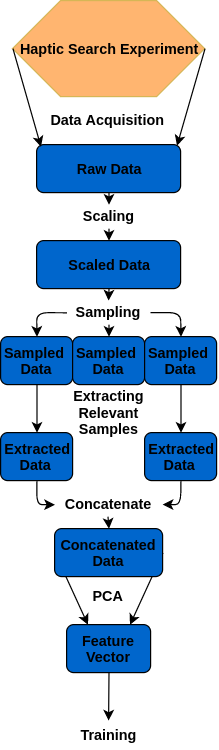
\includegraphics[scale]{Pipeline2}
	\makebox[\textwidth][c]{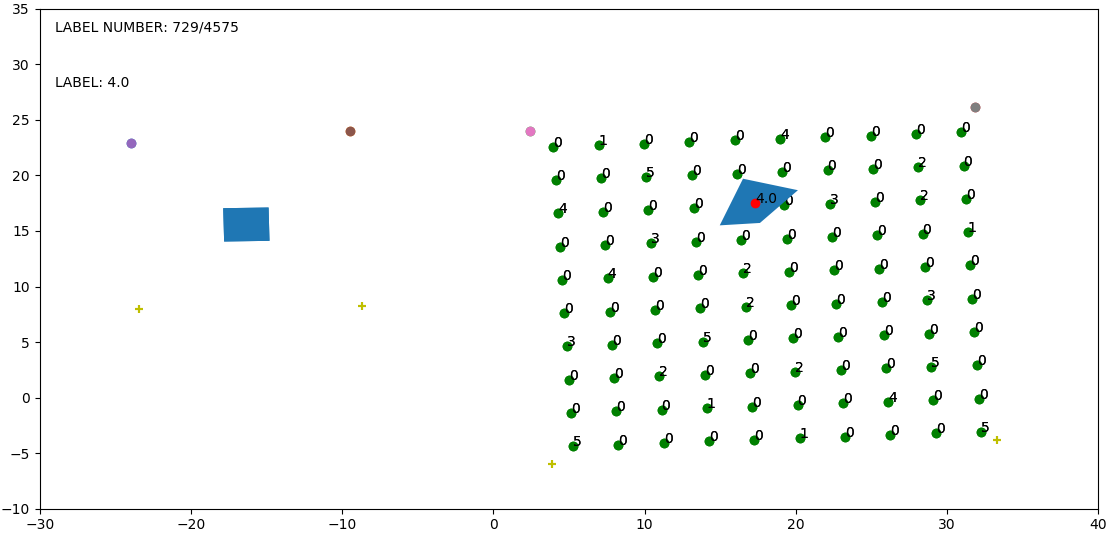
\includegraphics[width=\textwidth]{auto_label}}
	\caption{Auto-labeling visualization tool with the hand representation (blue polygon), the target object (blue square) and the search stimuli represented as their polygon center (green dots) and their respective labels.}
	\label{auto_label}
\end{figure}

A small addition was made after the first few observations. As a result of using only the center of the polygon, small noise in the position led to false labels when the center appeared to be closer to a neighbor object. To fix this problem, and additional parameter $ \gamma $ was added describing an attraction variable. If the same label occurs consecutively, meaning an object is explored for some duration, $ \gamma $ increases. When then the label changes, but the old one is still near, the algorithm will stick to the previous one while decreasing $ \gamma $. This ensures to avoid gaps of false labels.\\
\\
After generating the label vectors for the trials, almost no additional work had to be done manually. However if the data was too noisy, few gaps had to be filled by hand with the help of the visualization tool or good guessing.

%----------------------------------------------------------------------------------------
\section{Analyzing the Data}
For this experiment a total of seven subjects participated, each in up to five trials. After postprocessing the Vicon data, fitting a hand model and labeling, some problems were noticeable that led to an exclusion of trials from the final data set.\\
One problem was the loss of markers during an experiment. While most of these scenarios were detected and the trial was repeated, a few cases went unnoticed until the postprocessing step. It was not possible to reconstruct the hand model with less markers anymore.\\
A second problem was to much noise that would act as ghost markers in later processing steps. The programs used were able to handle just a specific amount of noise, so that a few trials could not be labeled.\\
\\
The final data set consists of data from \textbf{29} out of \textbf{35} trials and includes \textbf{137123} data points. Also included are the non relevant labels that describe cases where the hand was not exploring an object or outside the MHSB. In the table below the number of trials and data points for each participant A to G are listed:   

\begin{align}
	\label{database}
	\begin{tabular}{||c||c|c|c}
		\hline
		\multicolumn{3}{|c|}{Composition of the Dataset} \\
		\hline
		Participant & Trials & Data points \\
		\hline\hline
		A & 3 & 13867 \\
		B & 3 & 13887 \\
		C & 4 & 21230 \\
		D & 5 & 25720 \\
		E & 4 & 17895 \\
		F & 5 & 20446 \\
		G & 5 & 24078 \\
		\hline
	\end{tabular}
\end{align} 

An analysis of the sensor data revealed, that each participant had their own range of values, which most likely is correlated to their hand size and form. Smaller hands showed an slightly different area of activation for tactile data and also a significant different range for the joint angles. Due to this discovery, data from participants was treated separately rather than as one set. 